% -*- coding: UTF-8; -*-
\documentclass[11pt,onecolumn]{article}
%Pour langue et caract�res sp�ciaux
\usepackage[french]{babel} 
\usepackage[T1]{fontenc}
\usepackage{lmodern}
\usepackage[latin1]{inputenc}

\usepackage[top=2cm, bottom=2cm, left=2cm, right=2cm, columnsep=20pt]{geometry}   %Pour ajuster les marges
\usepackage{graphicx}      %pour inclure des graphiques
\usepackage{url}           %Pour inclure des adresse web
\usepackage{verbatim}      %pour inclure les codes en annexe, on utilisera la commande verbatim
\usepackage{amsmath}
\DeclareMathOperator{\Tr}{Tr}
\usepackage{cancel}
\usepackage{color}
\usepackage{mathrsfs}
\usepackage{amssymb}
\usepackage{mathtools}
\usepackage{xfrac}
\usepackage{float}
\usepackage{wrapfig}
\usepackage{framed}
\usepackage{subcaption}
\usepackage{listings}
\lstset{
basicstyle=\small\ttfamily,
columns=flexible,
breaklines=true
}

\renewcommand{\baselinestretch}{1.5} 

\begin{document}

%Page titre
\begin{titlepage}
\center

\vspace*{2cm}

\textsc{\LARGE Universit� de Montr�al}\\[1cm] 
\textsc{\Large IFT6269 - Probabilistic Graphical Models}\\[1.5cm] 

\rule{\linewidth}{0.5mm} \\[0.5cm]
{\LARGE \bfseries Homework 3} \\[0.2cm] % Titre page titre
\rule{\linewidth}{0.5mm} \\[3cm]

\large by: \\*
Patrice B�chard\\*
20019173\\[8cm] 


{\large \today}\\[3cm]

\vfill
\end{titlepage}

\section{DGM}

The implied factorization for the directed graphical model $G$ for any joint distribution $p(x_V) \in \mathcal{L}(G)$ is given by:

\begin{equation}
p(x_{_V}) = \prod_{i=1}^{N} p_i(x_i\mid x_{\pi_i}) = p(x)p(y)p(z| x,y) p(t | z)
\end{equation}
 
It is \textbf{not} true that $X \perp Y \mid T$ for any $p \in \mathcal{L}(G)$. We have seen in class that

\begin{equation*}
\boxed{\text{if } p \in \mathcal{L}(G) \Leftrightarrow X_A \perp X_B \mid X_C \; \forall \; A,B,C \text{ s. t. \textit{A} \& \textit{B} are \textbf{d-separated} by \textit{C}}}
\end{equation*}

We have also seen the definition of \textbf{d-separation}:

\begin{framed}
\begin{quote}
Sets \textit{A} \& \textit{B} are said to be \textbf{d-separated} by \textit{C} iff all chains from $a \in A$ to $b \in B$ are blocked given \textit{C}, where a chain from \textit{a} to \textit{b} is blocked at node \textit{d} if:

\begin{enumerate}

\item either $d \in C$ and $(v_{i-1}, d, v_{i+1})$ is not a v-structure.

\item $d \; \cancel{\in} \; C$, $(v_{i-1}, d, v_{i+1})$ is a v-structure and no descendents of \textit{d} is in \textit{C}.

\end{enumerate}
\end{quote}
\end{framed}

In our case, nodes \textit{X} and \textit{Y} are not d-separated by node \textit{T} since $(X,Z,Y)$ is a v-structure and \textit{T} is a descendent of \textit{Z}, which does not respect the second condition for v-separation.

\section{d-separation in DGM}

\begin{description}

\item (a) No
\item (b) Yes
\item (c) No
\item (d) Yes
\item (e) No
\item (f) No
\item (g) Yes
\item (h) No
\item (i) Yes
\item (j) No

\end{description}

\section{Positive interactions in-V-structures}

\begin{description}

\item (a)

\begin{description}
\item (i) For the condition $a > c$, let's use the following conditional probability tables:

\begin{table}[h]
\centering
	\begin{tabular}{c | c}
		X & p(x) \\
		\hline
		1 & 0.5 \\
		0 & 0.5
	\end{tabular}
\quad
	\begin{tabular}{c | c}
		Y & p(y) \\
		\hline
		1 & 0.5 \\
		0 & 0.5
	\end{tabular}
\quad
	\begin{tabular}{c c | c} 
		X & Y & p(Z=1 | x,y) \\
		\hline
		1 & 1 & 0.1 \\
		1 & 0 & 1 \\
		0 & 1 & 0.2 \\
		0 & 0 & 1
	\end{tabular}
\end{table}

We can now easily compute the different wanted values:

\begin{align}\label{eq:a}
a & = P(X=1) \\
	& = 0.5 \nonumber
\end{align}
\begin{align}\label{eq:b}
b = P(X=1 \mid Z=1) & = \frac{P(X=1, Z=1)}{P(Z=1)} \nonumber \\
				& = \frac{\sum_{i\in \{0,1\}} P(X=1)P(Y=i)P(Z=1 \mid X=1, Y=i)}{\sum_{i,j \in \{0,1\}} P(X=i)P(Y=j)P(Z=1 \mid X=i, Y=j)} \\
				& \approx 0.478 \nonumber
\end{align}
\begin{align}\label{eq:c}
c = P(X=1 \mid Z=1, Y=1) & = \frac{P(X=1, Z=1, Y=1)}{P(Z=1,Y=1)} \nonumber \\
					& = \frac{P(X=1)P(Y=1)P(Z=1 \mid X=1, Y=1)}{\sum_{i \in \{0,1\}} P(X=i)P(Y=1)P(Z=1 \mid X=i, Y=1)} \\
					& \approx 0.333 \nonumber
\end{align}

\item (ii) Now, for the condition $a < c < b$, let's use the following CPTs:

\begin{table}[h]
\centering
	\begin{tabular}{c | c}
		X & p(x) \\
		\hline
		1 & 0.5 \\
		0 & 0.5
	\end{tabular}
\quad
	\begin{tabular}{c | c}
		Y & p(y) \\
		\hline
		1 & 0.5 \\
		0 & 0.5
	\end{tabular}
\quad
	\begin{tabular}{c c | c} 
		X & Y & p(Z=1 | x,y) \\
		\hline
		1 & 1 & 1 \\
		1 & 0 & 0.5 \\
		0 & 1 & 0.5 \\
		0 & 0 & 0
	\end{tabular}
\end{table}

We can now easily compute $a$, $b$ and $c$ using equations \ref{eq:a}, \ref{eq:b} and \ref{eq:c}.

\begin{equation*}
a = 0.5
\qquad
b = 0.75
\qquad
c \approx 0.667
\end{equation*}

\item (iii) $b < a < c$

\begin{table}[h]
\centering
	\begin{tabular}{c | c}
		X & p(x) \\
		\hline
		1 & 0.5 \\
		0 & 0.5
	\end{tabular}
\quad
	\begin{tabular}{c | c}
		Y & p(y) \\
		\hline
		1 & 0.5 \\
		0 & 0.5
	\end{tabular}
\quad
	\begin{tabular}{c c | c} 
		X & Y & p(Z=1 | x,y) \\
		\hline
		1 & 1 & 1 \\
		1 & 0 & 0 \\
		0 & 1 & 0.1 \\
		0 & 0 & 1
	\end{tabular}
\end{table}

$a$, $b$ and $c$ can now be easily computed :

\begin{equation*}
a = 0.5
\qquad
b = 0.4
\qquad
c \approx 0.667
\end{equation*}

\end{description}

\item (b)

\begin{description}

\item (i) If the probability of $Z=1$ is slim if $Y=1$, then the probability of $X=1 \mid Z=1, Y=1$ will be smaller than the probability of $X=1$ alone.

\item (ii) If it is highly probable that we obtain $Z=1$ if $X=1$, then $b>a$. However, if the probability of having $Z=1$ given $Y=1$ is high as well, then the probability of having $X=1 \mid Y=1, Z=1$ will be lower than if we don't know the value of $Y$ yet.

\item (iii) If it is certain for event $Z$ to happen if both events $X$ and $Y$ happen at the same time or do not happen, but it is also possible for $Z$ to happen if $Y=1$ and $X=0$ in some rare cases (the opposite case where $Z=1$ when $X=1, Y=0$ is impossible). If we know that $Z$ happened, chances are $X$ and $Y$ happened (or did not happen) at the same time since the other option is a lot less probable. If we know that $Y=1$, it is almost certain that $X=1$ as well, but if we don't know the result of $Y$, the probability of $X=1\mid Z=1$ is just a bit less than the probability that $X=1$.

\end{description}

\end{description}

\section{Flipping a covered edge in a DGM}

We have that $\mathcal{L}(G) = \{p:p(x_{_V}) = p(i|\pi_i) p(j|\pi_i, i) p_*\}$ and $\mathcal{L}(G') = \{p:p'(x_{_V}) = p(i|\pi_i, j) p(j|\pi_i) p_*$, where $p_*$ represents the rest of the distribution, which is identical for both graphs. We can prove that the family of distributions represented by both of these graphs are identical by showing that the factorization of joint distribution is identical:

\begin{align*}
p(x_{_V}) & = p_* p(i|\pi_i)p(j|i,\pi_i) \\
		& = p_* \frac{\cancel{p(i,\pi_i)}}{p(\pi_i)}\frac{p(i,j,\pi_i)}{\cancel{p(i,\pi_i)}} && \text{(By definition)}\\
		& = p_* \frac{p(i,j,\pi_i)}{p(\pi_i)} \frac{p(j,\pi_i)}{p(j,\pi_i)} && \text{(Multiplying by 1)} \\ 
		& = p_* \frac{p(i,j,\pi_i)}{p(j,\pi_i)} \frac{p(j,\pi_i)}{p(\pi_i)} && \text{(Rearranging)} \\ 
		& = p_* p(i|j,\pi_i) p(j|\pi_i) && \text{(By definition)} \\
		& = p'(x_{_V}) \quad \blacksquare
\end{align*}

\section{Equivalence of directed tree DGM with undirected tree UGM}

For $G(V,E)$ a directed acyclic graph (DAG), we call $\bar{G}(V,\bar{E})$ the \textit{moralized graph} of $G$ where $\bar{G}$ is an undirected graph with the same nodes $V$ as $G$ and edges $\bar{E}$ given by:

\begin{equation*}
\bar{E} = \left\{ \{i,j\} : (i,j) \in E \right\} \cup \left\{ \{k,j\} : k \neq l \in \pi_i \text{ for some } i\right\}
\end{equation*}

In our case, since $G$ is a directed tree (does not contain v-structures), no additional edges appear, meaning that $\bar{E} = E$ (except for the fact that the edges are now undirected). For the moralized graph $\bar{G}$ obtained, the family of distributions represented by it are :

\begin{equation*}
\mathcal{L}(\bar{G}) = \left\{ p : \bar{p}(x_{_V}) = \frac{1}{Z} \prod_{c\in \mathcal{C}} \psi_c(x_c)  \right\}
\end{equation*}

where $\psi_c(x_c) \ge 0 \;\forall\; x_c$ are the \textit{potentials} and $Z = \sum_x \prod_{c \in \mathcal{C}} \psi_c(x_c)$ is the \textit{partition function}. Since the moralization of the directed tree $G$ did not yield any new edge, nodes are only fully connected 2x2, which means there is no new cliques formed. With $Z=1$, each potential representing the edge between two nodes in the undirected graph still represents the same probability as it was representing in its directed form :

\begin{equation*}
\psi_{\{a,b\}}(x_a,x_b) = p(b\mid a)
\end{equation*}

This yields $\bar{p}(x_{_V}) = p(x_{_V})$, and finally we get that $\mathcal{L}(G) = \mathcal{L}(\bar{G})$.

\section{Hammersley-Clifford Counter example}

For this problem, we consider a simple undirected 4-cycle graph ($X_1 - X_2 - X_3 - X_4 - X_1$), where each node is a binary random variable $X_i$ for $i \in \{1,2,3,4\}$. The probability distribution is $1/8$ for each of these configurations :

\begin{align*}
(0,0,0,0) \quad (0,0,0,1) \quad (0,0,1,1) \quad (0,1,1,1) \\
(1,1,1,1) \quad (1,1,1,0) \quad (1,1,0,0) \quad (1,0,0,0)
\end{align*}

and is $0$ for all other configurations. We can first show that the graph respects the global Markov property :

\begin{framed}
\begin{quote}
We say that \textit{p} satisfies \textit{global Markov property} with respect to undirected graph \textit{G} iff
\begin{equation*}
\forall \; A, B, S \subseteq V \text{ such that } S \text{ separates } A \text{ from } B \text{ in } G \text {, then } X_A \perp X_B \mid X_S
\end{equation*}

\end{quote}
\end{framed}

It is easy to see that for $p$ to satisfy global Markov property, we must have that $X_1 \perp X_3 \mid X_2, X_4$ and that $X_2 \perp X_4 \mid X_1, X_3$. The graph tells us that we should be able to interchange $X_1$ with $X_3$ as well as $X_2$ with $X_4$ and still obtain the same distribution, i.e. $p(x_1,x_2,x_3,x_4) = p(x_4,x_3,x_2,x_1)$. Developing for all possible configurations :

\begin{center}
\begin{tabular}{c @{\hskip 30pt} c}
$p(0,0,0,0) = p(0,0,0,0) = 1/8$ & $p(1,0,0,0) = p(0,0,0,1) = 1/8$ \\
$p(0,1,0,0) = p(0,0,1,0) = 0$ & $p(1,1,0,0) = p(0,0,1,1) = 1/8$ \\
$p(1,0,1,0) = p(0,1,0,1) = 0$ & $p(1,0,0,1) = p(1,0,0,1) = 0$ \\
$p(0,1,1,0) = p(0,1,1,0) = 0$ & $p(1,1,1,0) = p(0,1,1,1) = 1/8$ \\
$p(1,1,0,1) = p(1,0,1,1) = 0$ & $p(1,1,1,1) = p(1,1,1,1) = 1/8$
\end{tabular}
\end{center}

We notice that for whatever pair of values $(X_2,X_4)$ we choose, we know either $X_1$ or $X_3$ with certainty. If $(X_2,X_4) = (0,0)$, then $X_3 = 0$. If $(X_2, X_4) = (0,1)$, then $X_1 = 0$. If $(X_2, X_4) = (1,0)$, then $X_1 = 1$. Finally, if $(X_2,X-4) = (1,1)$, then $X_3 = 1$. This proves conditional independence between the $X_1$ and $X_3$ given $X_2, X_4$ for all possible cases.

We can finally prove that the distribution cannot be factorized in the way stated in the Hammersley-Clifford Theorem. Assuming that the distribution \textit{can} be factorized is such way, noting that the cliques in the graph are only the edges and absorbing the partition function $Z$, we have the following factorization :

\begin{equation*}
p(x_1,x_2,x_3,x_4) = \psi_{\{1,2\}}(x_1,x_2)\psi_{\{2,3\}}(x_2,x_3)\psi_{\{3,4\}}(x_3,x_4)\psi_{\{4,1\}}(x_4,x_1)
\end{equation*}

Knowing that the following equations are true :

\begin{align*}
p(0,0,1,0) = \psi_{\{1,2\}}(0,0) \psi_{\{2,3\}}(0,1) \psi_{\{3,4\}}(1,0) \psi_{\{4,1\}}(0,0) & = 0 \\
p(0,0,0,0) = \psi_{\{1,2\}}(0,0) \psi_{\{2,3\}}(0,0) \psi_{\{3,4\}}(0,0) \psi_{\{4,1\}}(0,0) & = 1/8 \\
p(0,0,1,1) = \psi_{\{1,2\}}(0,0) \psi_{\{2,3\}}(0,1) \psi_{\{3,4\}}(1,1) \psi_{\{4,1\}}(1,0) & = 1/8 
\end{align*}

This means that $\psi_{\{3,4\}}(1,0)$ must be 0. However, we also know that the following statement is true :

\begin{equation*}
p(1,1,1,0) = \psi_{\{1,2\}}(1,1) \psi_{\{2,3\}}(1,1) \psi_{\{3,4\}}(1,0) \psi_{\{4,1\}}(0,1)  = 1/8 
\end{equation*}

This yields a contradiction, so the distribution cannot be factorized according to $G$. $\blacksquare$

\section{[Bonus]: bizarre conditional independence properties}

\begin{equation*}
X \perp Y \mid Z \Leftrightarrow p(x,y \mid z) = p(x \mid z) p(y \mid z)
\qquad
X \perp Y \Leftrightarrow p(x,y) = p(x) p(y)
\end{equation*}

\begin{align*}
p(x,y\mid z) & = \frac{p(z \mid x,y) p(x,y)}{p(z)} && \text{by Bayes rule} \\
& = \frac{p(z\mid x,y) p(x) p(y)}{p(z)} && \text{by hypothesis} 
\end{align*}

We also have that :

\begin{align*}
p(x,y \mid z) & = p(x\mid z) p(y\mid z) && \text{by hypothesis} \\
 & = \frac{p(z \mid x) p(x)}{p(z)} \frac{p(z \mid y) p(y)}{p(z)} && \text{by Bayes rule} 
\end{align*}

Putting both expressions together, we get:

\begin{align*}
\frac{p(z \mid x) \cancel{p(x)}}{\cancel{p(z)}} \frac{p(z \mid y) \cancel{p(y)}}{p(z)} & = \frac{p(z\mid x,y) \cancel{p(x)} \cancel{p(y)}}{\cancel{p(z)}} \\ 
\frac{p(z \mid x)p(z \mid y)}{p(z)} & = p(z \mid x,y)
\end{align*}

\section{Implementation : EM and Gaussian mixtures}
\begin{description}

\item (a) The implementation of the K-means algorithm is found in the class \texttt{K\_Means} in the file \texttt{hwk3.ipynb}. We present various figures obtained with different random initializations for the cluster means as well as the final objective function values obtained after convergence for each case in figures \ref{fig:kmeans1}, \ref{fig:kmeans2} and \ref{fig:kmeans3}.

\begin{figure}[p!]
	\centering
	\begin{subfigure}[b]{0.5\textwidth}
		\centering
		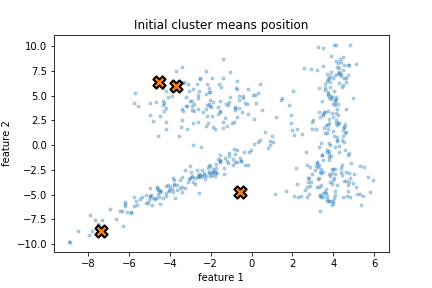
\includegraphics[scale=0.6]{figures/init_kmeans_00.png}
	\end{subfigure}%
	~
	\begin{subfigure}[b]{0.5\textwidth}
		\centering
		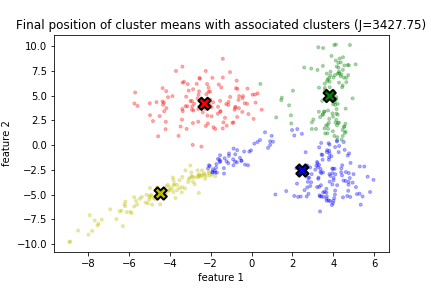
\includegraphics[scale=0.6]{figures/final_kmeans_00.png}
	\end{subfigure}
	\caption{\label{fig:kmeans1}\small{Random initialization of cluster means (left) and final cluster means with associated data point (right) using the K-means algorithm implementation. The final objective function value obtained is $J=3427.75$. }}
\end{figure}

\begin{figure}[p!]
	\centering
	\begin{subfigure}[b]{0.5\textwidth}
		\centering
		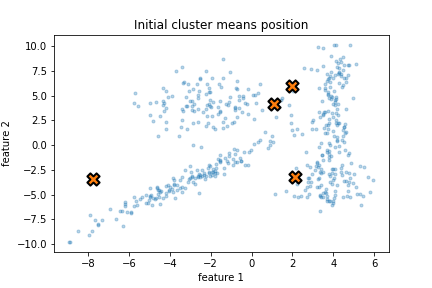
\includegraphics[scale=0.6]{figures/init_kmeans_01.png}
	\end{subfigure}%
	~
	\begin{subfigure}[b]{0.5\textwidth}
		\centering
		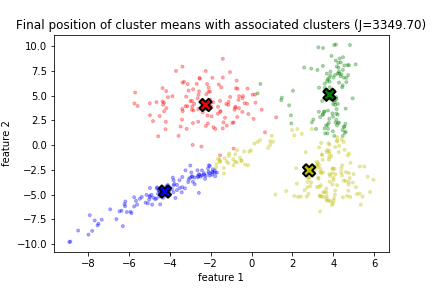
\includegraphics[scale=0.6]{figures/final_kmeans_01.png}
	\end{subfigure}
	\caption{\label{fig:kmeans2}\small{Random initialization of cluster means (left) and final cluster means with associated data point (right) using the K-means algorithm implementation. The final objective function value obtained is $J=3349.70$. }}
\end{figure}

\begin{figure}[p!]
	\centering
	\begin{subfigure}[b]{0.5\textwidth}
		\centering
		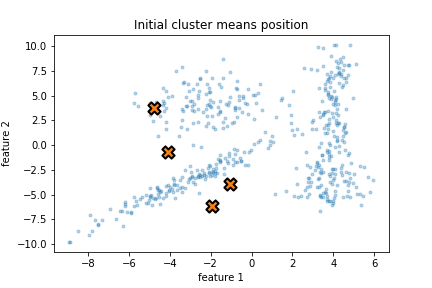
\includegraphics[scale=0.6]{figures/init_kmeans_02.png}
	\end{subfigure}%
	~
	\begin{subfigure}[b]{0.5\textwidth}
		\centering
		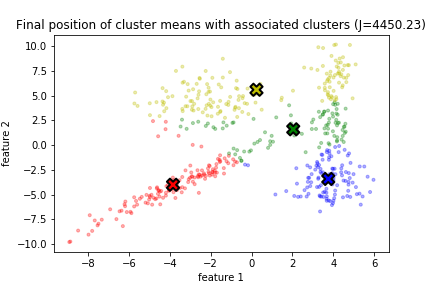
\includegraphics[scale=0.6]{figures/final_kmeans_02.png}
	\end{subfigure}
	\caption{\label{fig:kmeans3}\small{Random initialization of cluster means (left) and final cluster means with associated data point (right) using the K-means algorithm implementation. The final objective function value obtained is $J=4450.23$. }}
\end{figure}

\item (b) For a Gaussian mixture model, we have to optimize parameters $\theta = (\pi, \{\mu_j\}_{j=1}^{k}, \{\Sigma_j\}_{j=1}^{k})$. Knowing that the random variables $Z_{1:n}$ and $X_{1:n}$ are distributed as such :

\begin{equation*}
Z_i \sim \text{Mult}(\pi)
\qquad
X_i\mid Z_{i=j} \sim \mathcal{N}(\mu_j, \Sigma_j)
\end{equation*}

we have the complete log-likelihood given by:

\begin{align*}
\log p(x,z; \theta) & = \sum_{i=1}^{n} \left[ \log p(x_i\mid z_i; \theta) + \log p(z_i; \theta) \right] \\
			& = \sum_{i=1}^{n} \left[ \sum_{j=1}^{k} z_{i,j} \log \mathcal{N}(x_i \mid \mu_j, \Sigma_j) + \sum_{j=1} ^{k} z_{i,j} \log \pi_j \right] \\
\mathbb{E}_q \left[\log p(x,z;\theta)\right] & = \sum_{i=1}^{n} \sum_{j=1}^{k} \mathbb{E}_q[z_{i,j}]\left[ \log \mathcal{N}(x_i \mid \mu_j, \Sigma_j) + \log \pi_j \right]
\end{align*}

The E step of the EM algorithm consists of computing the weights $\tau_{i,j}^t$ for all i, j, which are given by:

\begin{align*}
\tau_{i,j}^t \triangleq p(z_{i,j}=1 \mid x_i, \theta_t) & = q_{t+1}(z_{i,j}=1) \\
									& = \frac{\pi_{j}^{(t)} \mathcal{N}(x_i \mid \mu_j ^{(t)}, \Sigma_j ^{(t)})}{\sum_{l=1}^{k} \pi_l ^{(t)} \mathcal{N}(x_i\mid \mu_l ^{(t)}, \Sigma_j ^{(t))}}
\end{align*}

Following the E step, the M step consists of finding the maximum likelihood estimator for each parameter using the weights $\tau_{i,j}^t$ instead of $\mathbb{E}_q[z_{i,j}]$ in the complete log-likelihood as such :

\begin{equation}\label{eq:max_expression}
\max_{\{\mu_j,\Sigma_j, \pi_j\}} \sum_{i=1}^{n} \sum_{j=1} ^{k} \tau_{i,j} ^{(t)} \left[ \log \mathcal{N}(x_i \mid \mu_j, \Sigma_j) + \log \pi_j \right]
\end{equation}

As usual, to maximize, we have to derivate the expression with respect to the wanted parameter and then set to 0. We first assume that the gaussians are spherical (i.e the covariance matrix is proportional to the identity matrix : $\Sigma_j = \sigma^2_j I$). We also assume that the terms $\tau_{i,j}$ are constant with respect to the parameter by which we derivate. To find the expression for $\pi_j$, we introduce the Lagrange multiplier $\lambda$, knowing that $\sum_{j=1}^{k} \pi_j = 1$, and we solve for $\pi_j$:

\begin{equation*}
\frac{\partial}{\partial \pi_j} \left[\sum_{i=1}^{n} \sum_{j'=1} ^{k} \tau_{i,j'} \left[ \cancel{\log \mathcal{N}(x_i \mid \mu_{j'}, \sigma_{j'}^2)} + \log \pi_{j'} \right] + \lambda \left( \sum_{j'=1}^{k} \pi_{j'} - 1\right)\right] = 0
\end{equation*}
\begin{align}\label{eq:pi_mid}
\sum_{i=1}^{n} \frac{\tau_{i,j}}{\pi_j} + \lambda & = 0 \nonumber \\
\sum_{i=1}^{n} \tau_{i,j} & = - \lambda \pi_j  \\
\sum_{j=1}^{k} \sum_{i=1}^{n} \tau_{i,j} & = \sum_{j=1}^{k} \lambda \pi_j \nonumber\\
\sum_{i=1}^{n} \sum_{j=1}^{k} \tau_{i,j} & = \lambda \sum_{j=1}^{k} \pi_j \nonumber
\end{align}

Noticing that both $\pi_j$ and $\tau_{i,j}$ summed over $j$ both equal 1, we find that $\lambda = -n$. We finally get the result we want, coming back to equation \ref{eq:pi_mid}:

\begin{equation}
\boxed{\hat{\pi}_j = \frac{1}{n}\sum_{i=1}^{n} \tau_{i,j}}
\end{equation}

We can now do the same for the mean $\mu_j$. Starting again from equation \ref{eq:max_expression}, we have:

\begin{align*}
\frac{\partial}{\partial \mu_j} \left[\sum_{i=1}^{n} \sum_{j'=1} ^{k} \tau_{i,j'} \left[ \log \mathcal{N}(x_i \mid \mu_{j'}, \sigma_{j'}^2) + \cancel{\log \pi_{j'}} \right]\right] & = 0 \\
\sum_{i=1}^{n} \frac{\partial}{\partial \mu_j} \left[ \sum_{j'=1} ^{k} \tau_{i,j'} \left[ \cancel{-\frac{d}{2}\log 2\pi\sigma_{j'}^2} - \frac{1}{2\sigma_{j'}^2}(x_i-\mu_{j'})^T(x_i-\mu_{j'}) \right]\right] & = 0 \\
\sum_{i=1}^{n} \frac{1}{\sigma_{j}^2} \tau_{i,j} (x_i-\mu_j) & = 0
\end{align*}

Separating into two distinct summations and cancelling the $\sigma_{j}^2$'s, we have :

\begin{align}
\sum_{i=1}^{n} \tau_{i,j} x_i & = \sum_{i=1}^{n}  \tau_{i,j} \mu_j \nonumber \\
\Aboxed{\hat{\mu}_j & = \frac{\sum_{i=1}^{n} \tau_{i,j} x_i}{\sum_{i=1}^{n} \tau_{i,j}}}
\end{align}

Finally, let's do the same thing for $\sigma_j^2$, the last parameter to maximize. 

\begin{align*}
\frac{\partial}{\partial \sigma_j^2} \left[\sum_{i=1}^{n} \sum_{j'=1} ^{k} \tau_{i,j'} \left[ \log \mathcal{N}(x_i \mid \mu_{j'}, \sigma_{j'}^2) + \log \pi_{j'} \right]\right] & = 0 \\
\sum_{i=1}^{n} \frac{\partial}{\partial \sigma_j^2} \left[\sum_{j'=1}^{k} \tau_{i,j'} \left[-\frac{d}{2}\log 2\pi \sigma_{j'}^2 - \frac{1}{2}(x_i-\mu_{j'})^T(x_i-\mu_{j'})\left(\frac{1}{\sigma_{j}^{2}}\right)\right] \right]& = 0 \\
\sum_{i=1}^{n} \tau_{i,j}\left[ -\frac{d}{2\sigma_j^2} + \frac{(x_i-\mu_j)^T(x_i-\mu_j)}{2(\sigma_j ^2)^2} \right] & = 0 
\end{align*}

Multiplying both sides by $2 \sigma_j^4$, we obtain :

\begin{align}
\sum_{i=1}^{n} \tau_{i,j}\left[ -d\sigma_j^2 + (x_i-\mu_j)^T(x_i-\mu_j) \right] & = 0 \nonumber \\
\sum_{i=1}^{n} \tau_{i,j} (x_i-\mu_j)^T(x_i-\mu_j) & = \sum_{i=1}^{n} \tau_{i,j}d\sigma_j^2 \nonumber \\
\Aboxed{\hat{\sigma}_j^2 = \frac{\sum_{i=1}^{n} \tau_{i,j} (x_i-\mu_j)^T(x_i-\mu_j)}{d\sum_{i=1}^{n} \tau_{i,j}}}
\end{align}

We are now ready to implement the gaussian mixture model with the EM algorithm for spherical gaussians. The class \texttt{GMM} of the file \texttt{hwk3.ipynb} does precisely that for both the spherical gaussian (covariance matrix proportional to identity) and the full covariance matrix. Figures \ref{fig:iso1}, \ref{fig:iso2} and \ref{fig:iso3} presents the data and the cluster means after initialization using k-means clustering on the right and the clustering obtained using the gaussian mixture model with the EM algorithm on the right. We present the ellipse containing $95.45\%$ of the mass of the Gaussian distribution (2 standard deviations) as well as  the most likely latent variables for all data points.

\begin{figure}[p!]
	\centering
	\begin{subfigure}[b]{0.5\textwidth}
		\centering
		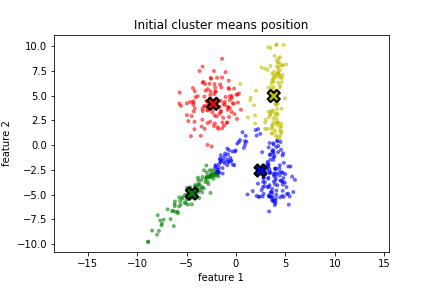
\includegraphics[scale=0.6]{figures/init_isotropic_00.png}
	\end{subfigure}%
	~
	\begin{subfigure}[b]{0.5\textwidth}
		\centering
		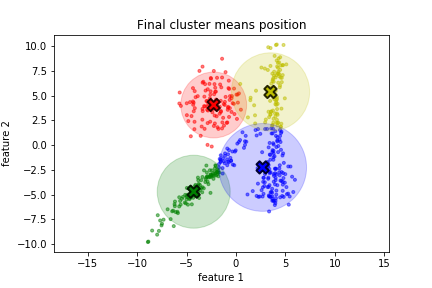
\includegraphics[scale=0.6]{figures/final_isotropic_00.png}
	\end{subfigure}
	\caption{\label{fig:iso1}\footnotesize{Initialization of cluster means with K-means algorithm(left) and final cluster means with associated data point (right) using the gaussian mixture model and EM algorithm implementation using isotropic gaussians.}}
\end{figure}

\begin{figure}[p!]
	\centering
	\begin{subfigure}[b]{0.5\textwidth}
		\centering
		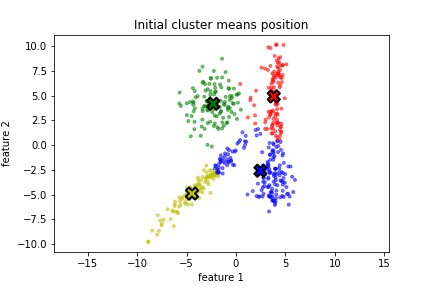
\includegraphics[scale=0.6]{figures/init_isotropic_01.png}
	\end{subfigure}%
	~
	\begin{subfigure}[b]{0.5\textwidth}
		\centering
		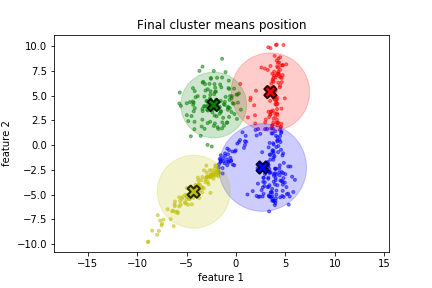
\includegraphics[scale=0.6]{figures/final_isotropic_01.png}
	\end{subfigure}
	\caption{\label{fig:iso2}\footnotesize{Initialization of cluster means with K-means algorithm(left) and final cluster means with associated data point (right) using the gaussian mixture model and EM algorithm implementation using isotropic gaussians. }}
\end{figure}

\begin{figure}[p!]
	\centering
	\begin{subfigure}[b]{0.5\textwidth}
		\centering
		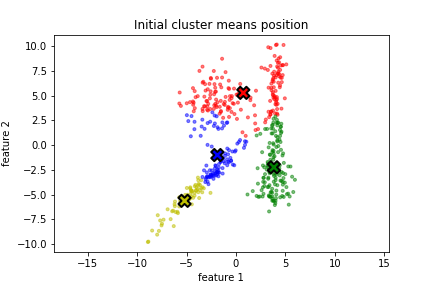
\includegraphics[scale=0.6]{figures/init_isotropic_02.png}
	\end{subfigure}%
	~
	\begin{subfigure}[b]{0.5\textwidth}
		\centering
		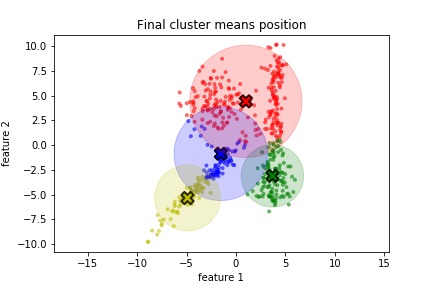
\includegraphics[scale=0.6]{figures/final_isotropic_02.png}
	\end{subfigure}
	\caption{\label{fig:iso3}\footnotesize{Initialization of cluster means with K-means algorithm(left) and final cluster means with associated data point (right) using the gaussian mixture model and EM algorithm implementation using isotropic gaussians.}}
\end{figure}

\item (c) Figures \ref{fig:full1}, \ref{fig:full2} and \ref{fig:full3} presents the data and the cluster means after initialization using k-means clustering on the right and the clustering obtained using the gaussian mixture model with the EM algorithm on the right. We present the ellipse containing $95.45\%$ of the mass of the Gaussian distribution (2 standard deviations) as well as  the most likely latent variables for all data points.

\begin{figure}[p!]
	\centering
	\begin{subfigure}[b]{0.5\textwidth}
		\centering
		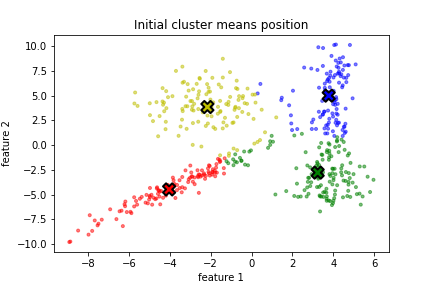
\includegraphics[scale=0.6]{figures/init_full_00.png}
	\end{subfigure}%
	~
	\begin{subfigure}[b]{0.5\textwidth}
		\centering
		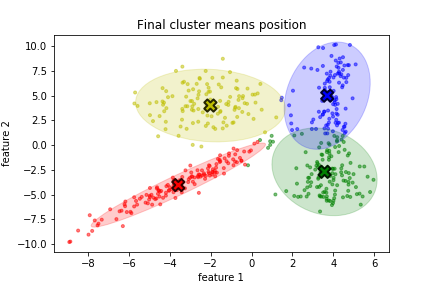
\includegraphics[scale=0.6]{figures/final_full_00.png}
	\end{subfigure}
	\caption{\label{fig:full1}\footnotesize{Initialization of cluster means with K-means algorithm(left) and final cluster means with associated data point (right) using the gaussian mixture model and EM algorithm implementation using gaussians with full covariance matrices.}}
\end{figure}

\begin{figure}[p!]
	\centering
	\begin{subfigure}[b]{0.5\textwidth}
		\centering
		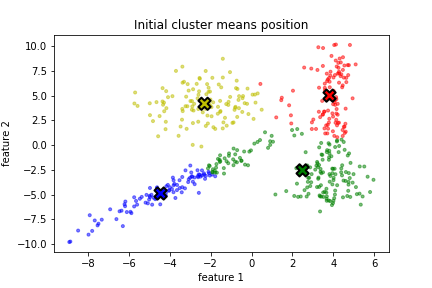
\includegraphics[scale=0.6]{figures/init_full_01.png}
	\end{subfigure}%
	~
	\begin{subfigure}[b]{0.5\textwidth}
		\centering
		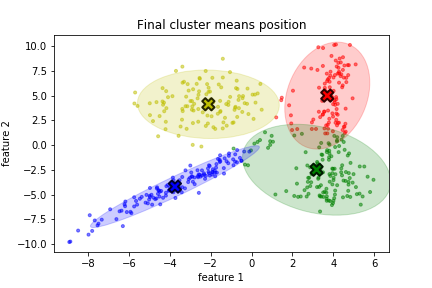
\includegraphics[scale=0.6]{figures/final_full_01.png}
	\end{subfigure}
	\caption{\label{fig:full2}\footnotesize{Initialization of cluster means with K-means algorithm(left) and final cluster means with associated data point (right) using the gaussian mixture model and EM algorithm implementation using gaussians with full covariance matrices. }}
\end{figure}

\begin{figure}[p!]
	\centering
	\begin{subfigure}[b]{0.5\textwidth}
		\centering
		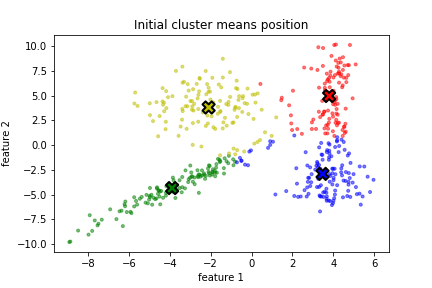
\includegraphics[scale=0.6]{figures/init_full_02.png}
	\end{subfigure}%
	~
	\begin{subfigure}[b]{0.5\textwidth}
		\centering
		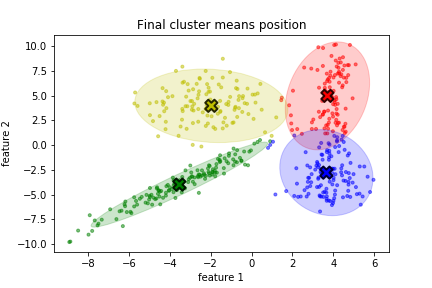
\includegraphics[scale=0.6]{figures/final_full_02.png}
	\end{subfigure}
	\caption{\label{fig:full3}\footnotesize{Initialization of cluster means with K-means algorithm(left) and final cluster means with associated data point (right) using the gaussian mixture model and EM algorithm implementation using gaussians with full covariance matrices. }}
\end{figure}

\item (d) By looking at the different plots generated, we can easily see that the best model for the data is the gaussian mixture model with full covariance matrix, which constantly returns really similar results, while the other models return results that differ depending on the initialization.

We can compare the normalized log-likelihood of the two mixture models on the training data found in the file \texttt{EMGaussian.train} as well as the test data found in \texttt{EMGaussian.test}. Knowing that the a cost function largely used in unsupervised learning is $-\log p(X;\Theta)$, we thus know that the smaller is this value on the test data, the better our model is. Table \ref{tab:loglikelihood} presents the results obtained for each mixture model implemented.

\begin{table}[h]
\centering
\begin{tabular}{c | c | c}
 & Isotropic covariance matrix & Full covariance matrix \\
 \hline
 Training data & 5.43 & 4.85 \\
 Test data & 5.38 & 4.99
\end{tabular}
\caption{\label{tab:loglikelihood}\small{Negative normalized log-likelihood obtained with both mixture models that were implemented.}}
\end{table}
\end{description}

We see that the model using full covariance matrix is better than the other, obtaining a smaller negative normalized log-likelihood than the other model. We also see that both model do not tend to overfit the data, getting a similar negative normalized log-likelihood for both the training data and the test data in both cases.

It would be interesting in the future to implement the k-mean++ initialization of the cluster means to obtain more consistent and precise results.

\end{document}